\section{The chamber as built: bow and edges}\label{sec:asbuilt}
\sectionstate{partial}{bow: \texttt{rerun/model\_audit/followups/fb\_bow\_maps/} (\texttt{results\_final}), figure
\texttt{papers/paper1\_v2/figs/make\_bow.py} (reproduces \texttt{summary\_paper.json}); edge: \texttt{rerun/paper1\_figs/README.md}
(\texttt{edge\_study.py}, \texttt{edge\_angles.py}). v2 2026-11-10: the old sections 7.5 and 7.6. The bow is one page here, with a
figure drawn from data; the alternatives, the stability and the transfer to the beam are \cref{app:bow}.}
\intent{A TPC assumes a flat readout plane and a drift field normal to it. Neither holds to a millimetre, in two
measured ways: every readout board is bowed, and the field fringes at the two sides without passivation. Both set how
the tracking numbers are obtained: the first through a correction, the second through the fiducial.}

\subsection{The readout boards are bowed}\label{sec:bow}
A TPC converts the time structure of its signals into a track angle under two assumptions: that the readout plane is
flat, and that the drift field is perpendicular to it. On all five chambers both fail at the millimetre level, in the
way a bowed readout board predicts. Three observables show it.

\emph{Positions.} A track of slope $\tan\theta$ crosses a mesh displaced by $h$ along the drift direction at a point
shifted by $h\tan\theta$. The slope of the position residual against the slope of the reference track is therefore the
local height of the mesh, $h(x,y)$, measured independently by the X and the Y strips. \Crefp{fig:bow}{a, b} shows it
for chamber~A: a dish, lower at the centre than at the rim, in both directions and in both views. A quadratic surface
fitted to all tracks puts the centre $1.31\pm0.22$\,mm below a point 150\,mm out for chamber~A, and between 1.7 and
1.9\,mm for the other four (\crefp{fig:bow}{c}). The centre is the part further from the cathode, the direction in which
the weight of the board, the overpressure of the gas and the tension of the mesh all push.

\emph{Drift direction.} If the drift lines leave the mesh normal to its surface, charge made at a height $d$ above it
arrives displaced by $d\,\partial h/\partial x$, and the fitted transverse rate acquires an offset
$w_0=\vd\,r_f\,\partial h/\partial x$, with $r_f$ between $1/2$ for a flat cathode and 1 for a cathode bowed with the
board. For a dish, $w_0$ must ramp linearly across the chamber, with a slope fixed by the curvature measured from the
positions. It does, in all ten chamber views, with $r_f$ between 0.52 and 1.00 (\crefp{fig:bow}{d}). The sign is
predicted by the geometry, not fitted.

\emph{Cluster width.} The cluster of strips is narrowest for a track that runs along the local drift lines. This uses
amplitudes only, no times and no fitted angle, and the angle of the narrowest cluster moves across the chamber with
the predicted sign in all ten views, beyond two standard deviations in eight.

The bow is a static property of each chamber: nineteen runs, on other nights, in the other slot of the bench
and at other voltages, all give their chamber's depth within two standard deviations. A bow of the reference planes
could imitate the position signal but not the other two, and its contribution to the depth is bounded at
$0.4\pm0.2$\,mm (\cref{app:bow}).

For the reconstruction the bow is a correction, part of each chamber's calibration: a surface per chamber for the
drift direction and the height of the track point. It improves the angular resolution by a median of 16\,\% over the
ten views, tested on tracks held out of its fit; for chamber~A from 1.10 to 0.99\textdegree{} in X and from 1.07 to
0.90\textdegree{} in Y. The position residual improves by 5 to 18\,\%.
\askDylan{One new caveat, from the agent that rebuilt the figure. The bow fit has no position cut, and 7--15\,\% of its tracks
lie within 30\,mm of an unpassivated $x$ side, where the field fringes (\cref{sec:edge}). Without them the dish depths move
by at most 0.2\,mm (within $1\sigma$), but the X-view gradient of $w_0$ rises, and $r_f$ on X goes from 0.71 to 1.10 on
chamber~A and from 0.87 to 1.85 on chamber~C, outside the physical range. So ``$r_f$ between 0.52 and 1.00 on all ten views''
holds for the fit with the edges included. Either state that, or re-quote with the cut; it is your call. The depths and the
gain in resolution do not depend on it.}

\begin{figure}[tbp]
  \centering
  \figorbox{bow}{mesh height map and profiles of chamber A, dish depth of five chambers, closure}
  \caption{The bow of the readout plane, from the slope of the position residual against the slope of the reference
  track. (a) Chamber~A: height of the mesh in 70\,mm cells, X and Y strips combined, with the rigid tilt removed. (b)
  Chamber~A: the same quantity in bins along $x$ and along $y$ for tracks within 50\,mm of the centre line; filled, X
  strips; open, Y strips; lines, the quadratic surface fitted to all tracks (solid X, dashed Y). (c) Depth of the dish
  150\,mm from the centre for the five chambers: large markers, the combined value with its error; small markers, its
  four terms (X strips filled, Y strips open; along $x$, then along $y$). (d) Measured gradient of the drift-direction
  offset $w_0$ against the gradient predicted from the curvature of the mesh, for the ten chamber views; dashed,
  $r_f=1$; dotted, $r_f=1/2$; filled X, open Y.}
  \label{fig:bow}
\end{figure}

\subsection{The field fringes at the unpassivated sides}\label{sec:edge}
The resistive strips end at the two $y$ sides, where their ends are passivated; the two $x$ sides, at strip
coordinates 0 and 398.6\,mm, are not (\cref{sec:design_choices}). Within 20 to 30\,mm of the $x$ sides the chamber
behaves differently, in three ways that share one depth (\cref{fig:edge}).

The X angle is biased. The fitted slope differs from the reference by up to 0.1--0.36 in $\tan\theta$ within 5 to
20\,mm of a side and by less than 0.01 beyond 30\,mm, with opposite signs on the two sides (chambers A, C and E): the
drift lines converge
inwards, so charge released near the cathode lands further inside than it started. The drift column is longer, by up
to 1.1\,\textmu s at 5 to 10\,mm from a side in chamber~A, with more charge on more strips: the edge strips collect
electrons from outside the strip area, over longer paths. And the efficiency reaches its plateau only 10 to 20\,mm
from an $x$ side, against about 5\,mm from a passivated $y$ side. The second of these uses no track model and the
other two use the reference. A fringe of this reach is what a gap of 28\,mm gives: the field of an open edge decays
with a length of about $g/\pi\approx9$\,mm, so three such lengths reach 30\,mm.

This is not the bow. The bow puts the mesh nearer the cathode at the rim and predicts a shorter column there, by 45
to 64\,ns; the fringe makes it longer. The shifts measured at the edges of the five chambers, between $-115$ and
$+78$\,ns, are the sum of the two.

The fringe sets the fiducial. Angles and positions are quoted at least 30\,mm from the $x$ sides. The passivated $y$
sides are sharp for the efficiency but not for the angle: a band 10 to 30\,mm from them keeps the full efficiency,
while its Y angle is 1.3 to 1.9 times worse than in the interior. The efficiency does not need a fiducial at all: over
the full active area it is 0.9 points lower than in the interior (\cref{sec:single}).
\askDylan{The angle numbers of \cref{sec:angle} use the interior as defined in \cref{sec:definitions}, 8\,mm from the $y$ sides, so
they include the band in which the Y angle is 1.3--1.9 times worse. Either the fiducial for angles becomes 30\,mm on every
side (and the numbers are re-derived; Y should improve), or this paragraph says that the 8\,mm was kept.}

\begin{figure}[tbp]
  \centering
  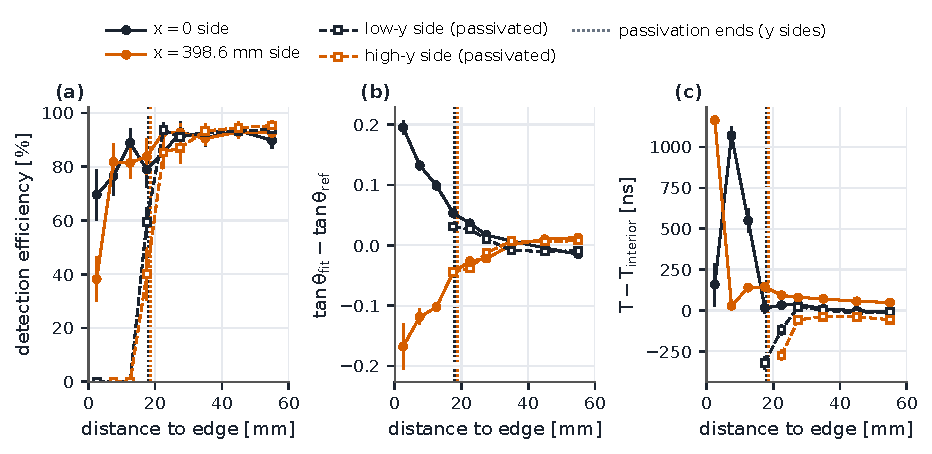
\includegraphics[width=\linewidth]{edge_turnon}
  \caption{Chamber~A near its sides, against the distance of the reference ray (or of the charge centroid in (c)) to
  the physical edge of the strip plane: (a) the efficiency, (b) the bias of the angle of the view perpendicular to the
  side, against the reference, (c) the duration of the drift column relative to the interior. Solid: the unpassivated
  $x$ sides; dashed: the passivated $y$ sides. Dotted vertical lines: where the passivation ends on the low-$y$
  (18.0\,mm) and high-$y$ (18.7\,mm) side. Error bars: binomial in (a); $1.25\,s_{68}/\sqrt{n}$ in (b). In (b), bins in
  which fewer than 30\,\% of the rays are detected are not shown; in (c) no trigger has its charge centroid in the
  passivated band.}
  \label{fig:edge}
\end{figure}
